    \subsection{Introduction}
    The Viola-Jones paper \cite{990517} describes a machine learning
    technique that achieves a fast and accurate object recognition
    method that does not base itself on deep learning. This report
    is still relevant today, especially for face detection and has
    been cited around 22,000 times. The technique used achieves
    itself from particular following three steps:
        \begin{itemize}
            \item The image reproduces itself using a summed-area
            table referred to as the integral image.

            \item The target object's principal features are picked
            out from a training set using an algorithm based on
            AdaBoost and generates efficient classifiers.
            
            \item The image passes into numerous filters, referred to
            as a "cascade structure" which is, in essence, a
            degenerate decision tree.  

        \end{itemize}

    This paper's detector was tested on 384 by 288 images at 15
    frames per second and accurate, irrelevant to facial features
    and ethnicity. The prompt detection of this technique is what
    makes it ahead of other methods.

    \subsection{The Integral Image}

        \subsubsection{Haar-Like Features}
        Haar-Like Features are rectangular points marked over an
        image, as shown in \ref{features} where the sum of pixels in
        the white rectangle subtracts from the grey rectangle's sum.
        By performing these calculations on raw image values, the
        result can take a significant amount of time. By calculating
        the integral image, these rectangular values can be performed
        quickly and in constant time. Figure \ref{ways} Shows
        different ways of calculating the features, (a) shows
        two-rectangle features, (b) shows three-rectangle features and
        (c) shows a four-rectangle feature.


    \begin{figure}[ht]
        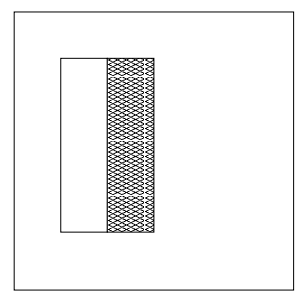
\includegraphics[scale=0.4]{sampleOne.png}
        \centering
        \caption{Shows an example of a Haar features}
        \label{features}
    \end{figure}


    \begin{figure}[H]
        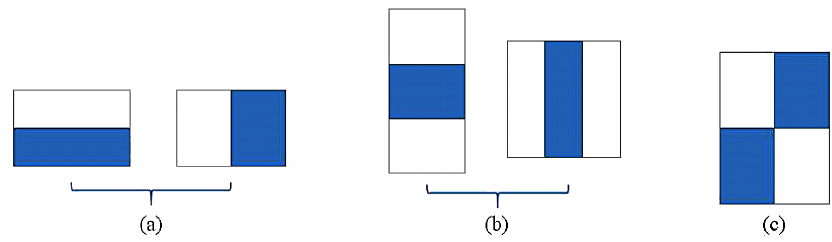
\includegraphics[scale=0.3]{features.png}
        \centering
        \caption{Different Ways of calculating Haar Features}
        \label{ways}
        
    \end{figure}

    \subsubsection{Calculating The Integral Image}
    The integral image is found by iterating over each pixel and
    computing its new value. This is obtained by calculating the sum
    of pixels above and to its left. The original pixel i(x,y)’s
    integral image ii(x,y) can be found using the following
    equation:

    \begin{center}
        \large{
            \(ii(x,y)= \sum_{(x \leq x,y' \leq y)}\)
        }
    \end{center}

    Example of original image and its integral image. 

    \begin{center}
        \begin{tabular}{ |c|c| }
            \hline
            1 & 5 \\ 
            \hline
            2 & 4 \\  
            \hline
        \end{tabular}

        Original Image
       \end{center}


       \begin{center}
            \begin{tabular}{ |c|c| }
                \hline
                1 & 6 \\ 
                \hline
                3 & 12 \\  
                \hline
            \end{tabular}

            Integral Image
        \end{center}


    % \subsubsection{Integral Image PseudoCode}

%             \begin{minted}[
%                 style=monokai,
%                 bgcolor=monokaibg
%             ]{python}
% for each pixel(x2,y2):
%     for x in [0,0] to x2:
%         for y in [0,0] to y2:
%             sum += Arr[x][y]
%             \end{minted}
%             \\ Where x1 is the row number of the top-left pixel [0,0], y1
%             is the column number of the top-left pixel [0,0], x2 is the
%             row number of the bottom-right pixel, y2  is the column
%             number of the bottom-right pixel.

            \subsubsection{Calculating the Sum of Any Pixel Value From the Integral Image}
            Consider the following matrix:
            \begin{figure}[ht]
                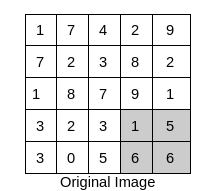
\includegraphics[scale=0.5]{photo1.png}
                \centering
            \end{figure}
            \\ The sum of the greyed out area is 1+5+6+6 which is
            \textbf{18}. Now consider its integral image:

            \begin{figure}[H]
                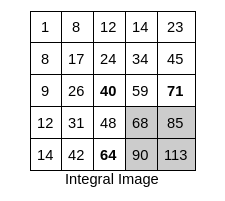
\includegraphics[scale=0.5]{photo2.png}
                \centering
            \end{figure}
            To Calculate the sum of the greyed out area subtract the
            summation of the unwanted areas's corner values, in this
            case: 
            \begin{center}
            113 - 64 - 71 which is  -22 as shown in figure
            \ref{cornerValues}.
            \end{center}

            \begin{figure}[H]
                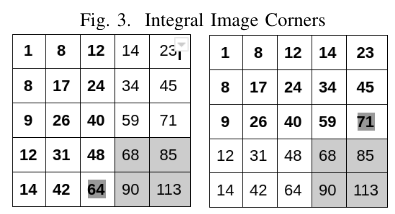
\includegraphics[scale=0.5]{cornerValues.png}
                \centering
                \caption{}
                \label{cornerValues}
            \end{figure}
            Then re-add the corner values of the areas that have been
            taken off twice in this case 
            \begin{center}
            +40 which results to \textbf{18}.
            \end{center}
            Although in this case, it did not make sense to calculate
            the integral image given how small the size of the
            original image is, in large pictures, this would save much
            time. 
    
            \subsection{Learning Classification Functions Using AdaBoost}
            Over 180,000 features can be calculated in an image given
            a small detector of size 24x24 pixels. This number of
            features results in both slow classification and
            overfitting. To avoid such problems a boosting algorithm
            (AdaBoost) \cite{freund1999short} is used to select a
            small set of critical Haar-like features using weak
            classifiers. For each of the features, the algorithm finds
            the function which separates them positively (contain a
            face) and negatively (do not contain a face) in the most
            optimal way ie. leaving the least possible number of
            values misclass Given a 24 by 24 image \(x\) with feature
            \(f_j\), a weak classifier \((h_j)\), is defined by 
            
            \begin{center}
                \(h_j(x)=1\) if \(p_j f_j < p_j\theta_j\) \\
                \(h_j(x)=0\) otherwise
            \end{center}
            where \(\theta_j\) is the treshold and \(p_j\) indicates
            the direction of the inequality sign.
 
        \subsubsection{Resultant Features}

            The figure shows the few numbers of features selected by
            AdaBoost. The two chief characteristics given priority are the
            darker eye area over the cheeks and the nose's bridge.


                \begin{figure}[H]
                    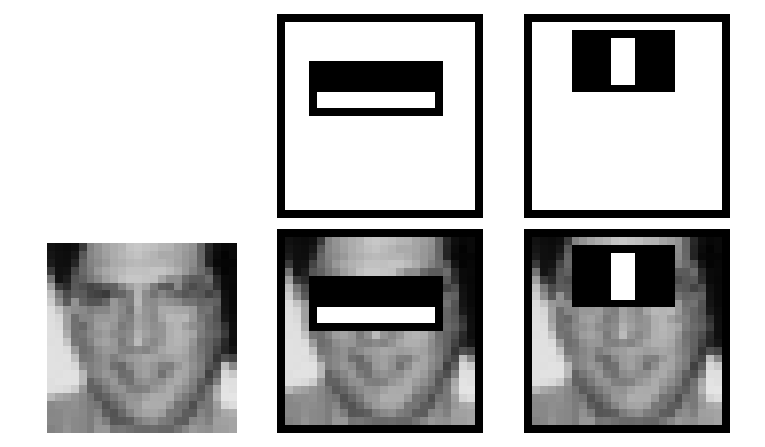
\includegraphics[scale=0.3]{selectedFeatures.png}
                    \centering
                    \caption{Some Resultant Features}
                    \label{resultantFeatures}
                \end{figure}           

            \subsection{Cascade of Classifiers}

                The third part of the algorithm places the previous
                features in the form of ranking stages where an image
                would have to pass through all of the stages which
                contain the object/face. By doing so, this increases
                performance by avoiding to count all the negative
                features. If the image fails to pass through the first
                feature, it fails.


            \begin{figure}[ht]
            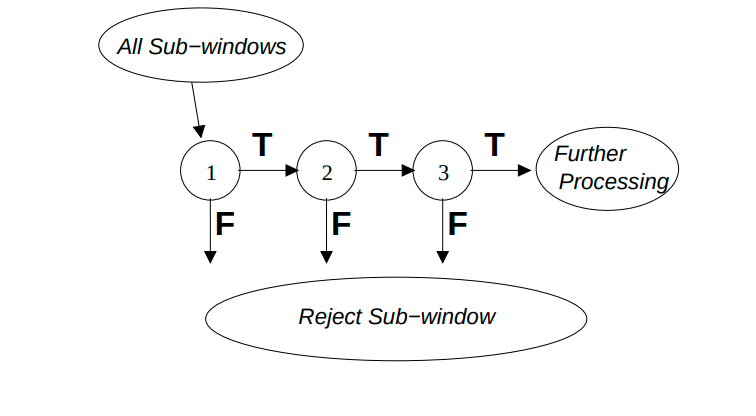
\includegraphics[scale=0.35]{cascade.png}
            \centering
            \end{figure}

            \subsection{Useful Applications for the Viola Jones algorithm}
            Although the modern standard approach for detecting
            objects is deep learning, the viola jones algorithm is
            still widely used today. The technique does not require
            much storage and can run on low powered devices and
            smartphones efficiently. That is why two modern real-life
            examples include several digital cameras, and the Snapchat
            face filters. \cite{Bansal}
